% we should list the event log definition and petri net definition
% also the process tree definition
% For definitions, we capitalize only the first character, others we use camel methods. 
This chapter introduces the most important concepts and notations that are used in this thesis. Firstly, the event data and process models typically used in process mining are described. Later, details of Inductive Miner techniques  are listed.
\section{Event Log}
% introduce of event and trace , later event log historical business process execution data in information systems
Business processes in organizations can be reflected by the execution of related activities. The historical execution data is usually stored as event logs in information systems and can be used by process mining techniques to analyze, understand, and improve the business execution. To specify the event log, we begin with formalizing  various notations \cite{van2016data} .
\begin{definition}[Event]
$\mathcal{A}$ is the universe of activities. An event $e$ for an activity  $a \in \mathcal{A}$ corresponds to one execution of this activity. The event set for a process is a finite set $\mathcal{E}$. 
\end{definition}
An event is characterized by attributes, like a timestamp, activity name, associated costs, etc. The executions of activities in a process are recorded as events. The set of events for a complete process case is a trace. Furthermore, the multiset of traces combines as an event log for the process. 


\begin{definition}[Trace and Event Log]
A trace $\sigma$ is a finite sequence of events, $\sigma \in \mathcal{E}^*$. An event log $L$ is a multiset of traces, $L \in \mathcal{B(\mathcal{E}^*)}$. 
\end{definition}
A trace also has a set of attributes, like its unique identifier, the cost. In this thesis, we extend this definition to handle traces with performance output according to certain KPIs. We call a trace labeled when this trace has a positive or negative label according to certain KPIs. Correspondingly, an event log is labeled if all of its traces have labels according to certain KPIs.
\section{Process Models}
After gathering an event log from information systems, process mining can discover a process model based on the event log. With this process model, the understanding of the business process can be improved. To describe the process, multiple process modeling languages are proposed in the past years, e.g, Petri net, BPMN models, etc. 

Among those model languages, Petri nets have been best studied thoroughly. Petri nets are capable to capture concurrent systems in a compact manner. Process trees are based on a tree structure to organize the event relation and simple to understand in comparison with other models, like BPMN models. In this thesis, Petri nets and process trees are used to represent our process.
\subsection{Petri Net}
A Petri net is a bipartite graph which consists of \textbf{\emph{transitions}} represented by a square and \textbf{\emph{place}} by a circle. \textbf{\emph{Tokens}} in black dots are put in places to express the dynamic states of a Petri net. An Petri net example is shown in Figure \ref{fig:pn-seq-2}. This Petri net is a workflow net with a token at the source place and satisfy the soundness conditions.  
\begin{figure}[!h]
	\centering
	\begin{subfigure}[b]{0.45\textwidth}
		\centering
		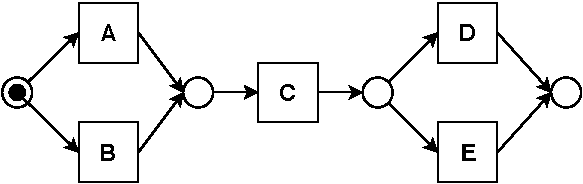
\includegraphics[width=\linewidth]{figures/preliminary/simple-petrinet.pdf}
		\caption{A simple Petri net}
		\label{fig:pn-seq-2}
	\end{subfigure}%
	\quad
	% here change the process tree into the transition system
	\begin{subfigure}[b]{0.5\textwidth}
		\centering
		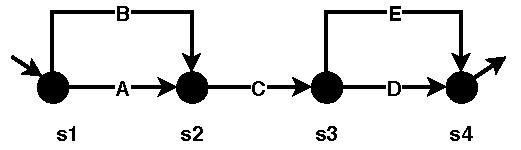
\includegraphics[width=\linewidth]{figures/preliminary/transition-system.pdf}
		\caption{A transition system corresponding to Fig \ref{fig:pn-seq-2}}
		\label{fig:ts-model}
	\end{subfigure}%
	\label{fig:pn-ts}
\end{figure}  

In the following, we define Petri nets in a formal way.
\begin{definition}[Petri net]
	A Petri net is a tuple $N=(P,T,F)$ where $P \cap T = \emptyset $. F is the set of arcs to connect places and transitions, $F \subseteq (P\times T)\cup (T \times P)$.
\end{definition}
Further, we can assign activity labels to transitions in Petri nets to describe the corresponding activities in business process. Usually, transitions with activity labels are seen \emph{observable actions}. To represent particular transitions that are not observable, we reserve label $\tau$ for them and name such transitions \emph{silent or invisible} transitions. A Petri net with labels are called labeled Petri nets and can be formalized in Definition \ref{def:labeled-PN}.
\begin{definition}[A labeled Petri net]\label{def:labeled-PN}	
	A labeled Petri net is a tuple $N=(P,T,F, \Sigma, \lambda)$, where $\Sigma$ is a set of activity labels, $\lambda$ is a function defined as $\lambda: T \rightarrow \Sigma \cup \tau$. A transition t with $\lambda(t)=\tau$ is a silent or an invisible transition.
\end{definition}
To express the dynamic states of Petri nets, we introduce a concept called \textbf{\emph{marking}} and extend the form  $N=(P,T,F)$ and define a marked Petri net. 
\begin{definition}[Marked Petri nets]
A marked Petri net is 4-tuple nets, $N=(P,T,F,M)$ where $M \in \mathbb{B(P)}$ is a place multiset called marking, which denotes the number of tokens in places.
\end{definition}
% we need to define the firing rules in Petri net. 
The firing sequence of transitions from Petri net corresponds to business execution in reality. A transition can be fired if it is in an enabled state where all the input places for this transition hold at least one token. After firing the transition, the token in the input places are consumed and new tokens are generated in the output places for this transition. Before we formalize the firing rule, we need several concepts below.
\begin{definition}[Input and output nodes]
	For a node $x$ in Petri net $N=(P,T,F)$, the set of its input nodes is denoted as $\bullet x = \{y\vert (y,x)\in F\}$. The set of its output nodes is denoted as $x\bullet = \{y\vert (x,y)\in F\}$.
\end{definition}
\begin{definition}[Firing rule]
	In a marked Petri net $N=(P,T,F,M)$, a transition $t\in T$ is enabled, written as $N[t\rangle$, if and only if $\bullet t \subseteq M$. After firing t, the marking changes in this way, $M \Rightarrow (M\setminus\bullet t)\cup t\bullet$.
\end{definition}
In real life, a subclass of Petri nets known as Workflow nets is often used to model business process.
\begin{definition}[Workflow nets]
	A workflow net is a labeled Petri net $N={P,T,F,\lambda}$ with constraints: 
	\begin{itemize}
		\itemsep-0.5em 
		\item P contains a source place denoted as $i$, where $ \bullet i=\emptyset$.
		\item P contains one sink place denoted as $o$, where $ o\bullet =\emptyset$.
		\item When connecting the sink place to source place by an arc, this net seen as a graph becomes strongly connected.
	\end{itemize}
\end{definition}   
However, not every Workflow net represents a correct process. To perform the business on an enterprise level, we define a minimum correctness criterion, known as soudness \cite{van2006structural}. 
\begin{definition}[Soundness]
	A Petri net is sound if and only if it satisfies the following conditions.
	\begin{itemize}
		\itemsep-0.5em 
		\item Safeness. Places cannot hold multiple tokens at the same time.
		\item Proper completion. If the sink place is marked, all other places are empty.
		\item Option to complete. It is always possible to reach the final marking from any reachable marking.
		\item No dead parts. For any transition, there exists a path from source to sink place through it. 
	\end{itemize}
\end{definition}

% should we give definitions about the redundant silent transitions and places here?? 
% When a Petri net with silent transitions, the model becomes complex to understand. The reduction of silent transitions and places should preserve the  behavior of the Petri net and keep the model sound. 

\subsection{Transition System}
%% Here add the definition for transitions system in Process mining
A transition system is a basic process model. As displayed in Figure \ref{fig:ts-model}, it is composed of \emph{states} and \emph{transitions}. \emph{States} are represented by black circles and include an initial and a final state. The initial state \textbf{s1} in Figure \ref{fig:ts-model} is denoted with an input arc without any label and the final state \textbf{s4} is with an output arc without label. \emph{Transitions}, also called actions, correspond to activities in the processes. They connect states by an arc.  
\begin{definition}[Transition System]
	A transition system is a triple $TS=(S,A,T)$ where S is the set of states, A is the set of activities, $T \subseteq S\times A\times S $ is the set of transitions, $(s_i, a, s_j) \in T$ is represented as $s_i \xrightarrow{a} s_j$.  
\end{definition}
Transition systems are eligible to describe the dynamic behavior and can easily be translated to Petri nets. The example models in Figure \ref{fig:ts-model} are mapped to each other. There are 5 transitions and four states in the transition system, which correspond to the transitions and places in Petri net. %Transition systems are simple but have difficulty to express concurrency in business process. So in our thesis, we use more expressive models like Petri nets to represent our process mining result.
\subsection{Process Tree}
Process tree is a tree and is suitable to represent a sound WF-net  by construction according to \cite{van2016data}. Moreover, as block-structured in a tree, process tree is easy to understand and use. Therefore, we introduce it in our thesis.
\begin{definition}[Process Tree]
Let $ A \subseteq \mathbb{A} $ be a finite set of activities with silent transition $\tau \notin \mathbb{A}$, $\bigoplus \subseteq \{\rightarrow, \times, \land, \circlearrowright\}$ be the set of process tree operators. 
\begin{itemize}
\item $Q=a$ is a process tree with $a\in A$, and 
\item $Q= \oplus (Q_1 , Q_2 ,.. Q_n)$ is a process tree with $\oplus \in \bigoplus$, and $Q_i$ is also a process tree, $ 1 \leq i \leq n$. 
\end{itemize}
\end{definition}
For convenience, given a process tree $Q= \oplus (Q_1 , Q_2 ,.. Q_n)$, we denote Q the parent for $Q_1 , Q_2 ,.. Q_n$, $Q_i$ as one child of Q. For a node in a tree without children, we call it a \textbf{\emph{leave node}}; Else, we call them \textbf{\emph{blocks}}.


Process tree operators represent different block relations of each subtree. Their semantics are standardized in  \cite{vanderAalst:2016:PMD:2948762, Buijs2012OnTR} and compared with Petri net in Figure \ref{fig:pn_pt_correspondings} \cite{Buijs2012OnTR}. We provide an informal description in the following.
\begin{figure}[!h]
	\centering
	\begin{subfigure}[b]{0.45\textwidth}
		\centering
		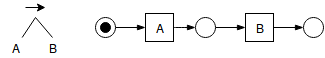
\includegraphics[width=\linewidth]{figures/preliminary/PT_PN_corresponding_01_seq_PN.png}
		\caption{Sequence}
		\label{fig:pt_pn_seq}
	\end{subfigure}%
	\quad
	\begin{subfigure}[b]{0.45\textwidth}
		\centering
		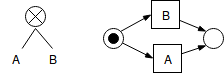
\includegraphics[width=\linewidth]{figures/preliminary/PT_PN_corresponding_02_xor_PN.png}
		\caption{Exclusive choice}
		\label{fig:pt_pn_xor}
	\end{subfigure}%
	\\ %this makes much difference
	\begin{subfigure}[b]{0.45\textwidth}
		\centering
		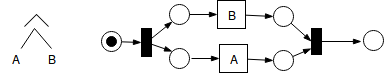
\includegraphics[width=\linewidth]{figures/preliminary/PT_PN_corresponding_03_and_PN.png}
		\caption{ Parallelism }
		\label{fig:pt_pn_and}
	\end{subfigure}%
	\quad
	\begin{subfigure}[b]{0.45\textwidth}
		\centering
		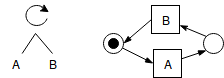
\includegraphics[width=\linewidth]{figures/preliminary/PT_PN_corresponding_04_loop_PN.png}
		\caption{Loop}
		\label{fig:pt_pn_loop}
	\end{subfigure}%
	\caption{Translation of process tree operators to Petri net}
	\label{fig:pn_pt_correspondings}
\end{figure}
\begin{definition}[Operator Semantics] 
	The semantics of operators $\bigoplus \subseteq \{\rightarrow, \times, \land, \circlearrowright \}$ are defined firstly in the context of its structure. The semantics with respect to a trace $\sigma$ are also given. 
		\begin{itemize}
		\item if $Q=(a)$, the tree only has one leaf node. 
		\item if $Q= \rightarrow(Q_1 , Q_2 ,.. Q_n)$, the subtrees have a sequential relation and are executed in order of $Q_1,Q_2,..Q_n$. 
		\item if $Q= \times(Q_1 , Q_2 ,.. Q_n)$,  the subtrees have an exclusive choice relation and only one subtree of $Q_1,Q_2,..Q_n$  can be executed. 
		\item if $Q= \land (Q_1 , Q_2 ,.. Q_n)$,  the subtrees have a parallel relation and $Q_1,Q_2,..Q_n$ they can be executed in parallel.
		\item if $Q= \circlearrowright(Q_1 , Q_2 ,.. Q_n)$,  the subtrees have a loop relation for $\{Q_1,Q_2,..Q_n\}$. $\{Q_2,..Q_n\}$ have an exclusive relation. $Q_1$ executes at first and is triggered again once one subtree of $\{Q_2,..Q_n\}$ executes. 
	\end{itemize}
\end{definition}
According to the corresponding semantic relations,  a process tree can be easily transformed into Petri net. In Figure \ref{fig:IM-split}, it is the process model in process tree which describes the same process as in Figure \ref{fig:pn-seq-2}. 

To describe the execution of  a process tree Q, we need concepts called \textbf{\emph{start nodes}} and \textbf{\emph{end nodes}}. The start nodes represent the firstly executed leaves nodes in Q; Similarly, the end nodes represent the last executed leaves node set in Q. 
\begin{definition}[Start node and end node set]
Given a process tree Q, its start node $S(Q)$ and end node set $E(Q)$ is defined as following. 
\begin{itemize}
	\item  $Q=(a) \quad \Rightarrow S(Q)=\{(a)\}=E(Q)$ ; 
	\item  $Q= \rightarrow(Q_1 , Q_2 ,.. Q_n) \Rightarrow S(Q)= S(Q_1); E(Q)=E(Q_n)$. The start node set is the start nodes of its first child, and the end node set is the end nodes from its last child.
	\item  $Q= \times(Q_1 , Q_2 ,.. Q_n) \Rightarrow S(Q)= \cup_{i\in \{1,..n\}}S(Q_i),E(Q)= \cup_{i\in \{1,..n\}}E(Q_i).$ \\For an exclusive choice block, its start and end node sets are the union of start and end nodes from each child; Any set from the union is an option start node set to represent the execution of Q. 
	\item $Q= \land (Q_1 , Q_2 ,.. Q_n) \Rightarrow S(Q)= \prod_{i} S(Q_i), E(Q)=\prod_{i} E(i)$. \\For parallel relation, the start nodes are all the start nodes from each child and end nodes are all the end nodes from each child.
	\item $Q= \circlearrowright(Q_1 , Q_2 ,.. Q_n) \Rightarrow S(Q)=S(Q_1), E(Q)=E(Q_1)$ \\The start node sets and end node sets depend on its first child.
\end{itemize}
\end{definition}

% here again the definition to address the relation. But it is executed due to several situations.
\iffalse
Given a sub process tree $Q= \oplus (Q_1 , Q_2 ,.. Q_n)$ and a trace $\sigma \in L$, we say that Q is executed by trace $\sigma$ from position i to j, if the activities corresponding to its start nodes set is executed from i and ends at j.
\begin{definition}[Execution of a process tree Q w.r.t. a trace $\sigma$ ]
 A process tree Q is executed according to a trace $\sigma$, if 
 \[\exists (a_1,a_2,...a_n)\in S(Q), \forall a_i, \exists j, \sigma(j)= a_i \]
\end{definition}
\begin{itemize}
	\item if $Q=a$, the beginning nodes for Q is a;
	\item if $Q= \rightarrow(Q_1 , Q_2 ,.. Q_n)$, the beginning nodes for Q are  subtrees have a sequential relation and are executed in order of $Q_1,Q_2,..Q_n$
	\item if $Q= \times(Q_1 , Q_2 ,.. Q_n)$,  the subtrees have an exclusive choice relation and only one subtree of $Q_1,Q_2,..Q_n$   can be executed.
	\item if $Q= \land (Q_1 , Q_2 ,.. Q_n)$,  the subtrees have a parallel relation and $Q_1,Q_2,..Q_n$ they can be executed in parallel.
	\item if $Q= \circlearrowright(Q_1 , Q_2 ,.. Q_n)$,  the subtrees have a loop relation for $\{Q_1,Q_2,..Q_n\}$. $\{Q_2,..Q_n\}$ have an exclusive relation. $Q_1$ executes at first and is triggered again once one subtree of $\{Q_2,..Q_n\}$ executes.
\end{itemize}
\fi
%% here to describe the inductive miner 
\section{Inductive Miner}
Among multiple discovery techniques to mine a process model from an event log, Inductive Miner suits well our needs, because it guarantees the construction of a sound models, and is flexible and scalable w.r.t. event log. In this section, we explain its algorithms in details.
\subsection{Construct a Directly-Follows Graph}
At the start, an event log $L$ is scanned to extract the \emph{directly-follows relation} of events which describes the execution order of pair activities. We denote directly-follows relation in an event log by $>_L$. 
  
For example, given an event log \[L_{IM}=\{<a,c,d>^{20},<b,c,e>^{10},<a,c,e>^{20},<b,c,d>^{10}\},\] 
a is directly followed by b and c, denoted as $a >_L b, a>_L c$; d directly follows b and c, $b>_L d, c>_L d$.

later, those directly-follows relations are combined together to build a directly-follows graph with frequency. According to  \cite{van2016data, leemans2013discovering}, formal definitions for the concepts above are given.
\begin{definition}[Directly-follows Graph]
 The directly-follows relation $a >_L b$ is satisfied iff \[\exists\sigma \in L, 1 \leq i < \vert \sigma \vert , \sigma(i)=a \ and \ \sigma(i+1)=b.\]
 A directly-follows graph of an event log $L$ is $G(L) = (A, F , A_{start}, A_{end}) $ where $A$ is the set of activities in L, $ F=\{ (a,b) \in A \times A | a >_L b \} $ is the directly-follows relation set, $A_{start}, A_{end}$ are the set of start and end activities respectively, $A_{start}=\{a\vert \exists \sigma \in L, a=\sigma(1)\}, A_{end}=\{a\vert \exists \sigma \in L, a=\sigma(\vert \sigma\vert)\}$.
\end{definition}
What's more, the frequency information of the directly-follows relation is stored to express the relation strength and denoted as cardinality. 
\begin{definition}[Cardinality in a directly-follows graph]
Given a directly-follows graph $G(L)=(A, F , A_{start}, A_{end})$ derived from an event log L, the cardinality in G(L) is defined respectively on the $F$, $A_{start}$, and $A_{end}$.  
	\begin{itemize}
		\itemsep-0.5em
		\item $\forall (a,b)\in F, c(a,b)=\sum_{\sigma \in L} |\{ i\in \{1,2...|\sigma|\} \vert \sigma(i)=\sigma(i+1)\} | $ is the frequency for directly-follows relation $a>_L b$. 
		\item $\forall a \in A_{start}, c(a)=\sum_{\sigma \in L} |\{\sigma \vert \sigma(1) = a\}|$ is the frequency for a start activity.
		\item $\forall a \in A_{end}, c(a)=\sum_{\sigma \in L} |\{\sigma \vert \sigma(|\sigma|) = a\}|$ is the frequency for an end activity.
	\end{itemize}	
\end{definition}
According to definitions above, we obtain a directly-follows graph from event log $L_{IM}$ as shown in the Figure \ref{fig:IM-dfg}. Cardinality information is listed on the connections of activities.
\begin{figure}[!h]
	\centering
	\begin{subfigure}[b]{0.4\textwidth}
		\centering
		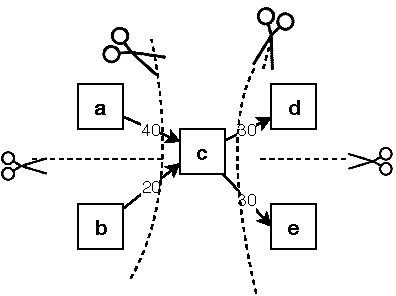
\includegraphics[width=\linewidth]{figures/preliminary/IM-demo-directly-follows.pdf}
		\caption{The directly-follows graph from $L_{IM}$. \small{The cut on directly-follows graph is shown in dashed line.}}
		\label{fig:IM-dfg}
	\end{subfigure}%
	\quad
	\begin{subfigure}[b]{0.55\textwidth}
		\centering
		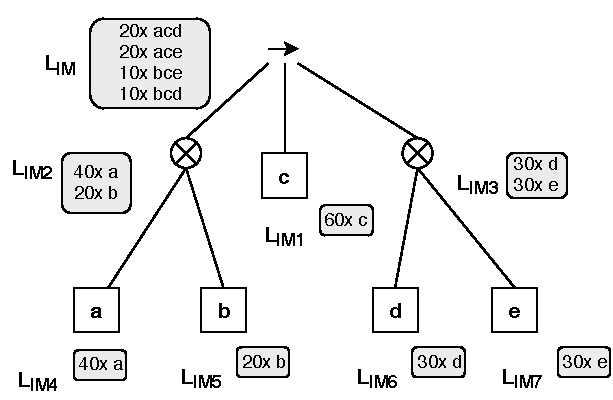
\includegraphics[width=\linewidth]{figures/preliminary/IM-demo-split-procedure.pdf}
		\caption{IM to split $L_{IM}$ for building a process tree}
		\label{fig:IM-split}
	\end{subfigure}%
	\\ %this makes much difference
	\caption{Inductive Miner to discover a process tree from event log $L_{IM}$}
	\label{fig:IM-demo}
\end{figure}
\subsection{Split The Event Log Into Sublogs}
Based on the directly-follows graph, the Inductive Miner finds the most prominent cut which is applied afterwards to split the event log into smaller sublogs. Corresponding to process tree operators $ \{\rightarrow, \times, \land, \circlearrowright \}$, cuts consist of \emph{exclusive-choice cut, sequence cut, parallel cut and redo-loop cut}. They are selected in the following order. A maximal exclusive-choice cut is firstly tried to split the directly-follows graph; if it is not available, then a maximal sequence cut, a  maximal parallel cut and a redo-loop cut are applied in sequence. As a result, sublogs are generated based on those cuts. Meanwhile, the operators which corresponds to those cuts are used to build the process tree. The same procedure is applied again on the sublogs until single activity set.  

As an example, we apply the splitting on event log $L_{IM}$ and $G(L_{IM})$ illustrated in Figure \ref{fig:IM-split}. Firstly, the $\rightarrow$ cut is applied and divides the whole event log into three sublogs $L_{IM1},L_{IM2},L_{IM3}$. Since $L_{IM1}$ includes only one single activity, so we stop splitting and build a corresponding node in the process tree. Next, $L_{IM2},L_{IM3}$ are split by exclusive choice cuts separately until meeting single set in $L_{IM4},L_{IM5},L_{IM6},L_{IM7}$.

Furthermore, a process tree is able to be converted into Petri net. 
